Während die Fresnelsche und die Fraunhofersche Beugung die zwei \glqq{}klassischen\grqq{} Zugänge zur Theorie der Beugung bilden, ist die Fourieroptik ein weiterer Ansatz zu diesem Gebiet, welcher sich die mathematischen Werkzeuge der Fourieranalyse zunutze macht. Im Versuch 233 (bzw. 333) werden wir die Beugung von Licht am Einzel- und Doppelspalt vor dem Hintergrund der Fourieroptik betrachten.

\subsection{Physikalische Grundlagen}

\subsubsection*{Die Fraunhofersche Beugung}

Die Fresnelsche Beugung geht von endlichen Abständen zwischen Lichtquelle, Beugungsobjekt und Beobachtungsebene aus. Es treffen hierbei also Lichtstrahlen in verschiedensten Winkeln auf das Beugungsobjekt, entsprechend welcher sie gebeugt werden. Da die mathematische Beschreibung dieses Prinzips augenscheinlich sehr kompliziert ist, beschränken wir uns in diesem ersten Teil auf die Fraunhofersche Beugung.

Wie in \abbref{fig:fraunhofer_beugung} dargestellt, geht die Fraunhofersche Betrachtung der Beugung von unendlich großen Abständen zwischen Lichtquelle, Beugungsobjekt und Beobachtungsebene aus. In dieser Annäherung (\textit{bzw. Distanzierung lol}) treffen die Lichtstrahlen von der Quelle daher parallel und senkrecht auf das Beugungsobjekt. Da die gebrochenen Lichtbündel daher ebenfalls parallel sind, würden diese erst im Unendlichen interferieren (\ref{fig:fraunhofer_beugung}, links). Durch die Positionierung einer Sammellinse zwischen Beugungsobjekt und Beobachtungsebene (\ref{fig:fraunhofer_beugung}, rechts) lassen sich die Interferenzmuster bereits in der Entfernung der Brennweite der verwendeten Linse beobachten.

\begin{figure}[H]
  \centering
  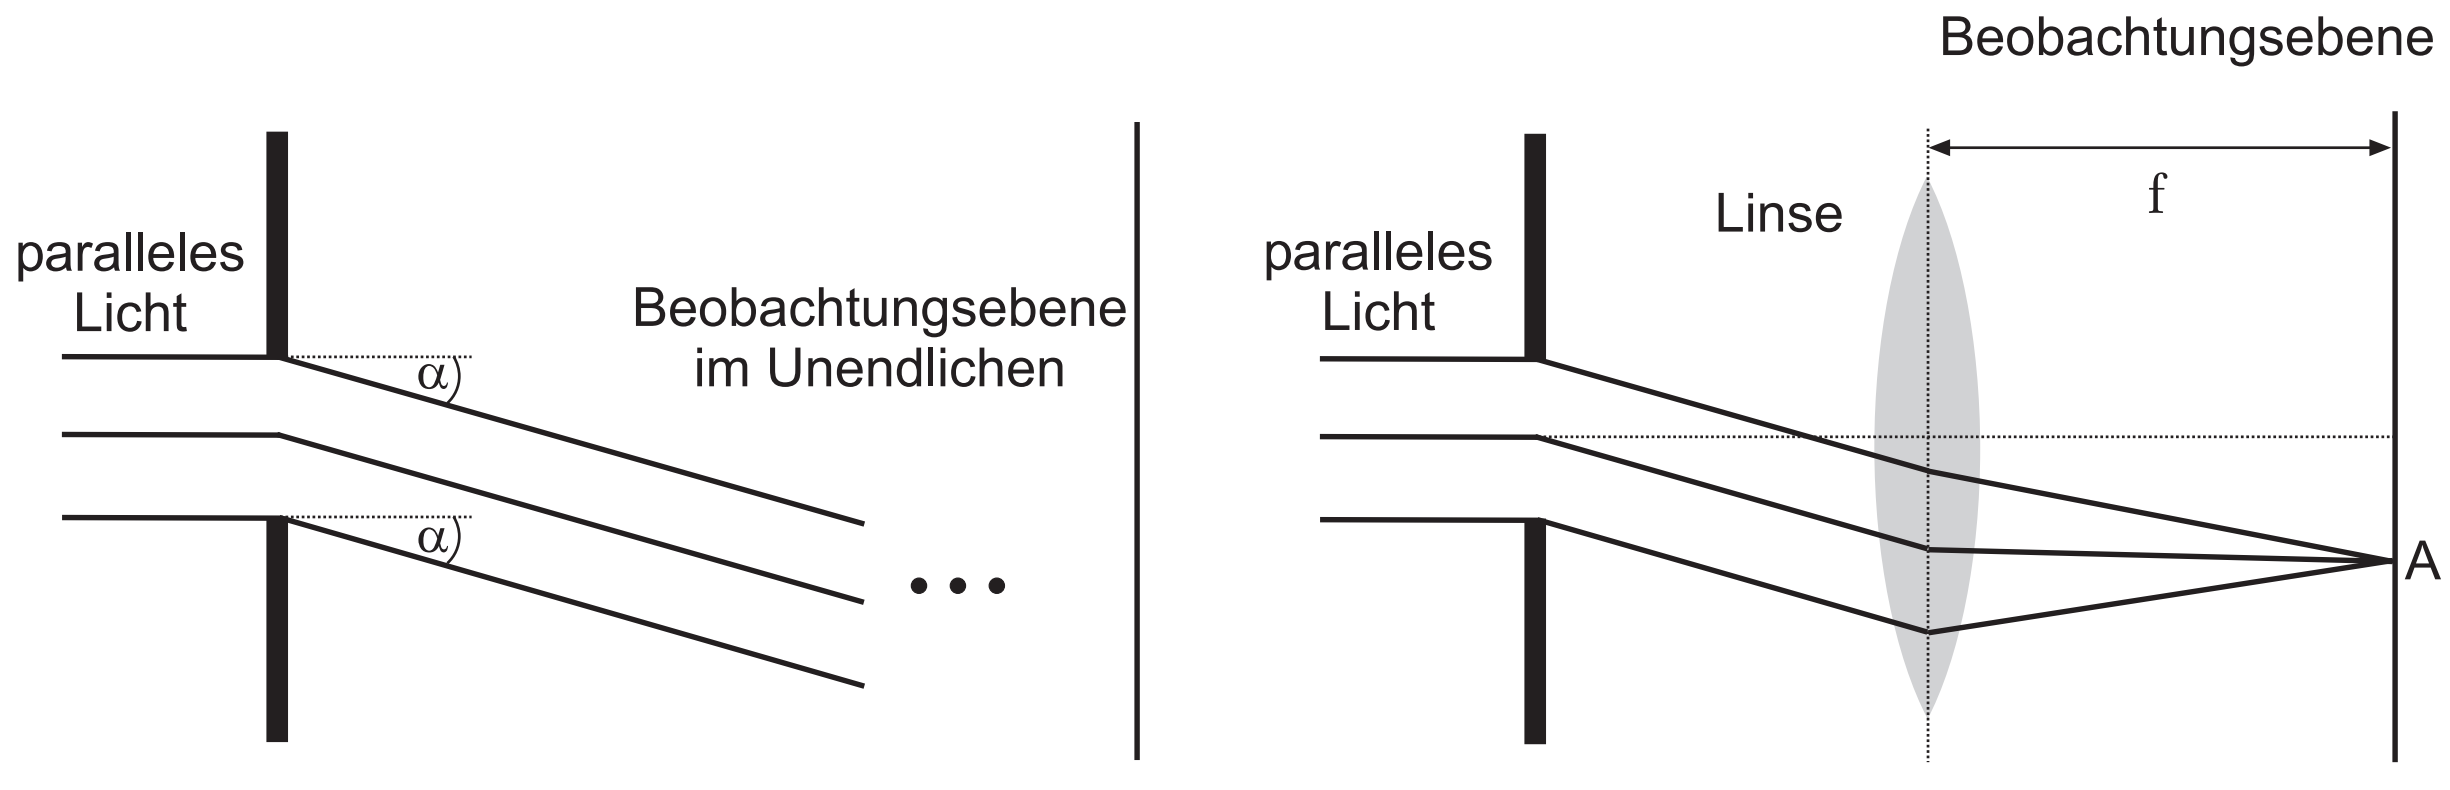
\includegraphics[width=.9\textwidth]{files/fraunhofer_beugung.png}
  \caption{Fraunhofersche Beugung mit Beobachtungsebene im Unendlichen (links) und in endlichem Abstand durch Verwendung einer Linse (rechts).}
  \label{fig:fraunhofer_beugung}
\end{figure}

Wir gehen nun von einem Spalt der Breite $d$ in y-Richtung, und einer Länge deutlich größer als $d$ aus. Alle Punkte des Spalts werden mit gleicher Amplitude $E_0$ und Phase $\varphi = \omega t$ von einem parallelen monochromatischen Lichtstrahl der Wellenlänge $\lambda$ erregt. Es gilt also
\begin{align}
  E(y) = E_0 \e{i\omega t}.
\end{align}

Das Huygens-Fermat'sche Prinzip besagt nun, dass von jedem dieser Punkte eine Elementarwelle ausgeht. Das Interferenzmuster dieser Wellen können wir bestimmen, indem wir die Überlagerung aller in einen bestimmten Winkel $\alpha$ ausgehenden Wellen betrachten. Mathematisch entspricht dies dem Integral
\begin{align}
    E_{\infty}(\alpha) = \int_{-\flatfrac{d}{2}}^{+\flatfrac{d}{2}} E_0 \e{i(\omega t - kl)} \dd y
\end{align}
mit dem Betrag des Wellenvektors $k = \frac{2\pi}{\lambda}$. 

\begin{figure}[H]
  \centering
  \begin{minipage}{0.65\textwidth}
    Der Gangunterschied zwischen einem Lichtbündel aus dem Mittelpunkt ($y = 0$) des Spalts und einem Lichtbündel abseits von diesem entspricht gerade $y \sin(\alpha)$. Somit gilt für die Weglänge des äußeren Bündels
    \begin{align}
      l = R + \sin(\alpha)
    \end{align}
    mit $R$ als Weglänge des Bündels aus dem Mittelpunkt. 
  \end{minipage}\hfill
  \begin{minipage}{0.3\textwidth}
      \centering
      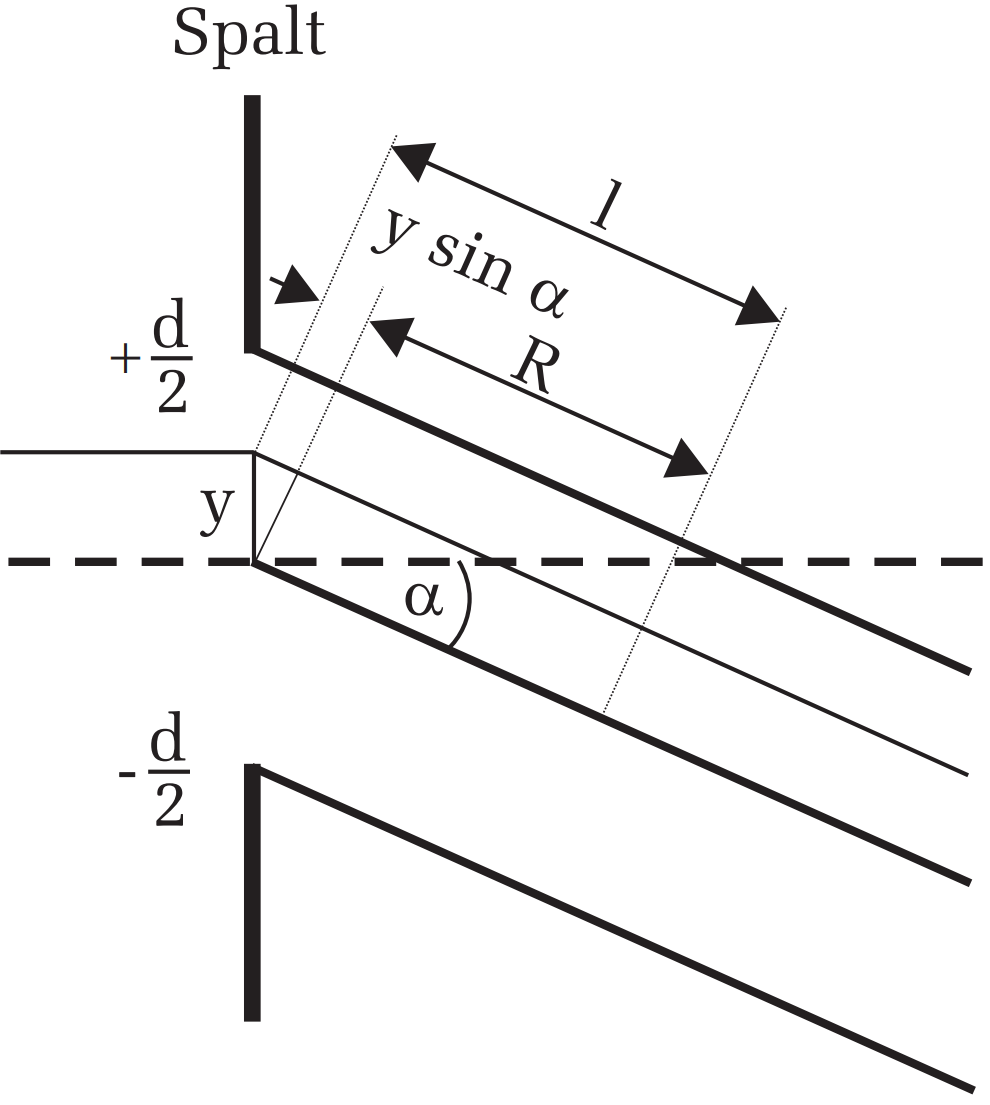
\includegraphics[width=0.9\textwidth]{files/gangunterschied_fraunhofer_einzelspalt.png}
      \caption{Gangunterschied der ausgehenden Lichtbündel am Einzelspalt.}
      \label{fig:gangunterschied_fraunhofer_einzelspalt}
  \end{minipage}
\end{figure}


Setzen wir diese Definition in das Integral ein, führen dieses aus und benutzen die Eulersche Formel für die e-Funktion, so ergibt sich
\begin{align}
  E_{\infty}(\alpha) = E_{0}\e{i(\omega t- kR)} \frac{\sin(\frac{\pi d \sin(\alpha)}{\lambda})}{\frac{\pi \sin(\alpha)}{\lambda}}.
\end{align}
\begin{figure}[H]
  \centering
  \begin{minipage}{0.55\textwidth}
    Wir identifizieren $x = \frac{d}{\lambda} \pi \sin(\alpha)$ und erhalten so
    \begin{align}
      E_{\infty}(x) = E_{0}\e{i(\omega t- kR)} \frac{\sin(x)}{x} d.
    \end{align}
    
    Durch das Quadrieren dieser Formel können wir die Intensität
    \begin{align}
      I_{\infty}(x) \propto \frac{\sin^2(x)}{x^2} d^2 \propto I_0 \frac{\sin^2(x)}{x}
    \end{align}
    mit $I_0 \propto d^2$ bestimmen. Diese ist dargestellt in \abbref{fig:intensitätsverteilung_fraunhofer_einzelspalt}.
  \end{minipage}\hfill
  \begin{minipage}{0.4\textwidth}
      \centering
      \includegraphics[width=0.9\textwidth]{files/intensitätsverteilung_fraunhofer_einzelspalt.png}
      \caption{Intensitätsverteilung der Beugungsstruktur des Einzelspalts.}
      \label{fig:intensitätsverteilung_fraunhofer_einzelspalt}
  \end{minipage}
\end{figure}

\subsubsection*{Fourierreihen und Fourierintegrale}

Eine Funktion $f: \R \to \R$ heißt periodisch, wenn ein $L \in \R$ existiert mit $f(x + L) = f(x)$ für alle $x \in \R$. Eine $L$-periodische und integrierbare Funktion lässt sich mit den trigonometrischen Funktionen
\begin{align}
  \cos(\frac{2\pi n}{L} x),\quad \sin(\frac{2\pi n}{L} x)\qquad n \in \N
\end{align}
als Basisvektoren entwickeln. Das heißt, es existieren $a_n, b_n \Forall n \in \N$ mit
\begin{align}
  f(x) = \frac{a_0}{2} + \sum_{n = 1}^{\infty} a_n \cos(\frac{2\pi n}{L} x) + b_n \sin(\frac{2\pi n}{L}) x.
\end{align}
Die sogenannten Fourierkoeffizienten $a_n$ und $b_n$ sind definiert durch 
\begin{align}
  a_n = \frac{2}{L} \int_{-\flatfrac{L}{2}}^{\flatfrac{L}{2}} f(x) \cos(\frac{2\pi n}{L} x) \dd x,
  \intertext{bzw.}
  b_n = \frac{2}{L} \int_{-\flatfrac{L}{2}}^{\flatfrac{L}{2}} f(x) \sin(\frac{2\pi n}{L} x) \dd x.
\end{align}

Zur Veranschaulichung können wir die Fourierkoeffizienten am Beispiel der Funktion
\begin{align}
  f(x) = \begin{cases}
    1, &-\ffrac{l}{2} < x < \ffrac{l}{2}\\
    0, &\ffrac{l}{2} > |x| < \ffrac{L}{2}
  \end{cases},
\end{align}
dargestellt in \abbref{}, ausrechnen.

Aus Symmetriegründen verfallen alle Koeffizienten $b_n$. Für $a_0$ gilt
\begin{align}
  a_0 = \frac{2}{L}\int_{-\ffrac{l}{2}}^{\ffrac{l}{2}} \dd x = \frac{2l}{L}.
\end{align}
Für alle weiteren $a_n$ gilt
\begin{align}
  a_n = \frac{2}{L} \int_{-l/2}^{l/2} \cos( \frac{2\pi n}{L} x ) \dd{x}
= \frac{1}{\pi n} \eval{ \sin( \frac{2\pi n}{L} x ) }_{-l/2}^{l/2}
= \frac{2}{\pi n} \sin( \pi n \frac{l}{L} ).
\end{align}

Setzen wir das Verhältnis $L:l = 2:1$, so erhalten wir die folgenden Summanden als erste Glieder der zugehörigen Fourierreihe:
\begin{align}
  f(x) = \frac{1}{2} 
+ \frac{2}{\pi} \cos( \frac{2\pi}{L} x ) 
- \frac{2}{3\pi} \cos( \frac{6\pi}{L} x ) 
+ \frac{2}{5\pi} \cos( \frac{10\pi}{L} x ) 
- \dots
\end{align}

\abbref{fig:fourierentwicklung_rechteck_beispiel} zeigt die Fourierentwicklung der Funktion für verschiedene, aufsteigende $n$ bis zu einem Wert von $n = 27$. Es ist zu sehen, dass die Linearkombination aus trigonometrischen Funktionen sich immer weiter der rechteckigen Form der Ausgangsfunktion annähert.

\begin{figure}[H]
  \centering
    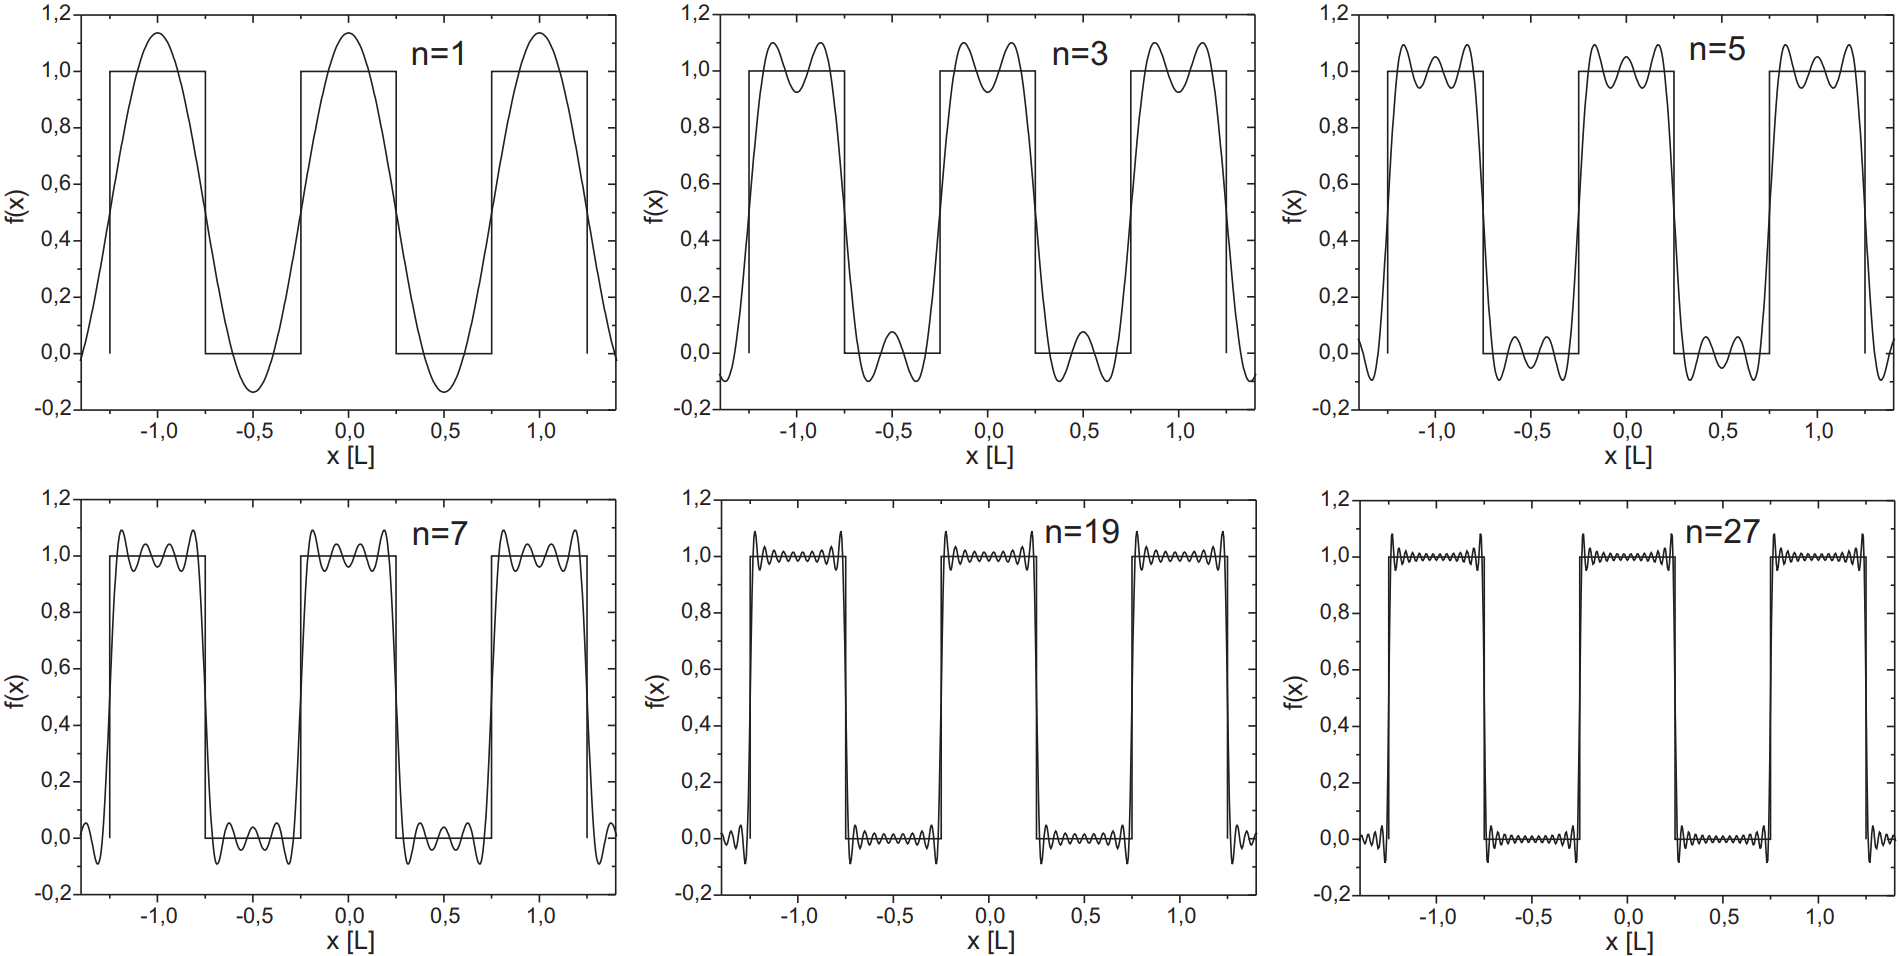
\includegraphics[width=0.9\textwidth]{files/fourierentwicklung_rechteck_beispiel.png}
    \caption{Fourierentwicklungen der gezeigten Rechtecksfunktion für verschiedene $n$.}
    \label{fig:fourierentwicklung_rechteck_beispiel}
\end{figure}

Die Gleichung
\begin{align}
  f(t) = \frac{a_0}{2} + \sum_{n=1}^{\infty} a_n \cos(n\omega t) + b_n \sin(n\omega t).
\end{align}
zeigt einen besonderen Anwendungsfall der Fourierentwicklung. Hier wurde $x$ durch die Zeit $t$ und die Periode $L$ durch die Periodendauer $T = \frac{2\pi}{\omega}$ mit der Frequenz $\omega$ ersetzt. In dieser Variante kann die Fourierreihe genutzt werden, um die verschiedenen anteiligen Frequenzen und Amplituden eines zeitperiodischen Signals zu ermitteln.

Während sie zwar nicht als Fourier\textit{reihe} dargestellt werden können, können wir auch nichtperiodische Funktionen dennoch mithilfe von trigonometrischen Funktionen darstellen. Für den Fall $L\to\infty$ geht die Fourierreihe in ein Integral und die Koeffizienten zu kontinuierlichen Funktionen über. Die kontinuierlichen Fouriertransformation ist dann definiert durch
\begin{align}
  f(x) = \int_{-\infty}^{\infty} F(k) \e{ikx} \dd k.
\end{align}

Dabei ist $F$ die Fouriertransformierte von $f$. Diese erhalten wir durch die Rücktransformation
\begin{align}
  F(k) = \frac{1}{2\pi} \int_{-\infty}^{\infty} f(x) \e{-ikx} \dd x.
\end{align}

Falls $x$ eine Ortsvariable ist, so nennen wir $k$ die Raum- oder Ortsfrequenz.

\subsubsection*{Die Fourierdarstellung der Fraunhoferbeugung}

Zu Herleitung der Fraunhoferschen Beugung aus der Fouriertheorie betrachten wir zunächst eine beliebige Öffnung $S$, wie sie in \abbref{fig:geometrie_herleitung_fourier_fraunhofer} dargestellt ist. Wir gehen davon aus, dass die Öffnung mit monochromatischem Licht bestrahlt wird, somit geht von jedem Flächenelement $\dd{S}(x = 0, y, z)$ eine Kugelwelle der Form 
\begin{align}
  \frac{\e{ikr}}{r}
\end{align}
mit der Quellstärke $\epsilon$ pro Einheitsfläche aus. Für das Feld am Ort $P$ in den Koordinaten $X,Y,Z$ gilt dann
\begin{align}
  \dd{E} = \epsilon \frac{\e{ikr}}{r} \dd{S}. \label{eq:dE_bei_P}
\end{align}
Der Abstand von $\dd{S}$ zu diesem Punkt $P(X,Y,Z)$ beträgt gerade
\begin{align}
  r = \sqrt{X^2 + (Y - y)^2 + (Z - z)^2}.
\end{align}
Der Abstand $R$ vom Mittelpunkt der Öffnung zum Punkt $P(X,Y,Z)$ beträgt
\begin{align}
  R = \sqrt{X^2 + Y^2 + Z^2}.
\end{align}
Damit können wir den Abstand $r$ umformen zu
\begin{align}
  r = R\sqrt{1 + \frac{(y^2 + z^2)}{R^2} - \frac{2 (Yy + Zz)}{R^2}}.
\end{align}

\begin{figure}[H]
  \centering
    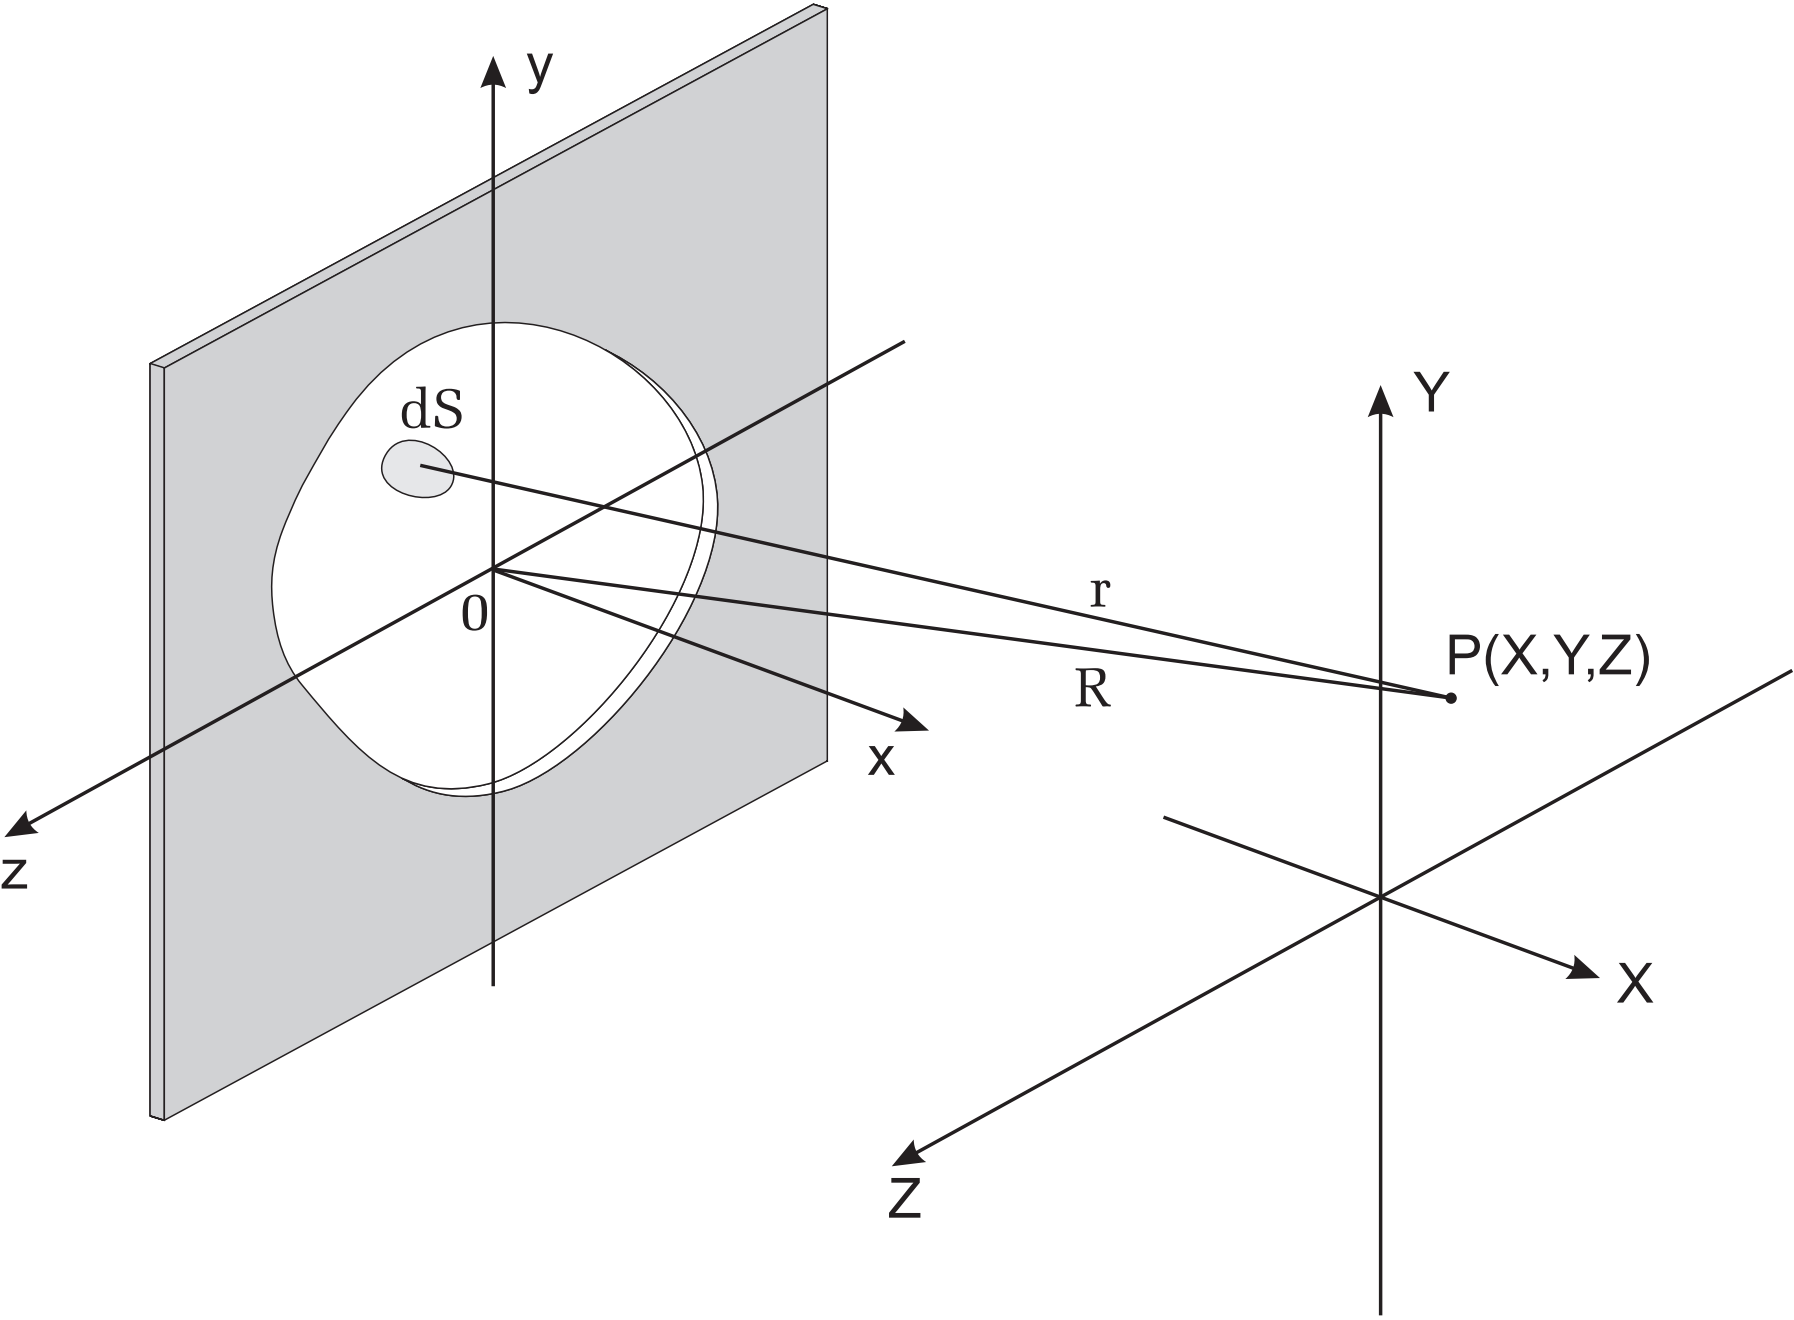
\includegraphics[width=0.8\textwidth]{files/geometrie_herleitung_fourier_fraunhofer.png}
    \caption{Geometrie des Spalts zur Herleitung der Fraunhoferbeugung aus der Fouriertheorie.}
    \label{fig:geometrie_herleitung_fourier_fraunhofer}
\end{figure}

Nun können wir annehmen, dass der Abstand $\overline{OP}$ deutlich größer gegenüber der Spaltöffnung ist. Dadurch gilt zum einen, dass wir $r$ im Amplitudenterm \eqref{eq:dE_bei_P} durch $R$ ersetzen können. Zum anderen gilt die Abschätzung
\begin{align}
  \frac{x^2 + y^2}{R^2} \ll 1
\end{align}
und somit
\begin{align}
  r = R \sqrt{1 - \frac{2(Yy + Zz)}{R^2}}
\end{align}

Gehen wir weiter davon aus, dass der Term in der Wurzel deutlich kleiner als $1$ ist, so können wir den Ausdruck weiter zu
\begin{align}
  r = R\qty(1 - \frac{Yy + Zz}{R^2})
\end{align}
vereinfachen. Diese Definition können wir nun ein Gleichung \eqref{eq:dE_bei_P} einsetzen und diese über die Gesamte Öffnung $S$ integrieren. So erhalten wir zunächst
\begin{align}
  E(R) = \epsilon \frac{\e{ikR}}{R} \int \int \e{-\frac{ik}{R}(Yy+Zz)} \dd{y} \dd{z}.
\end{align}

Nun nehmen wir zuerst die Annäherung vor, dass wir uns auf einen kleinen Bereich um $R$ beschränken und somit den Term $\ffrac{\e{ikR}}{R}$ als Konstant annehmen können. Weiter erweitern wir die Quellstärke $\epsilon$ um eine Abhängigkeit von $y$ und $z$, also
\begin{align}
  \epsilon \to \epsilon(y, z) = A(y,z) = A_0(y, z)\e{i\varphi(y,z)}.
\end{align}
Die \textit{Öffnungsfunktion} $A(y,z) \dd{y} \dd{z}$ ist proportional zum Feld der vom Flächenelement $\dd{y}\dd{z}$ ausgehenden Welle.  Mit dieser Definition ergibt sich das Integral
\begin{align}
  E(Y,Z) = \int\int_{S} A(y,z) \e{-\frac{ik}{r}(Yy + Zz)} \dy\dz.
\end{align}
Nun können wir die Raumfrequenzen durch
\begin{align}
  k_y = k\frac{Y}{R}, \qquad k_z = k \frac{Z}{R}
\end{align}
definieren. Setzen wir diese in das Integral
\begin{align}
  E(k_y, k_z) = \int\int_S A(y,z) \e{-i(k_y y + k_z z)} \dy \dz
\end{align}
ein, so erhalten wir gerade die \textbf{zweidimensionale Fouriertransformation der Öffnungsfunktion} $A(y,z)$.

\subsubsection*{Das Beugungsbild des Spalts als Fouriertransformierte der Spaltöffnung}

Als erste Anwendung der gerade erlangten Erkenntnisse betrachten wir die Öffnungsfunktion
\begin{align}
  A(y,z) = f(y) = \begin{cases}
    1, & |y| \leq \ffrac{d}{2},\\
    0, & |y| > \ffrac{d}{2}.
  \end{cases}
\end{align}
Die Fouriertransformation dieser Funktion lässt sich wie folgt ausrechnen:
\begin{align}
  F(k_y) &= \int_{-\infty}^{\infty} f(y) \e{-ik_y y} \dy\\
          &= \int_{-\ffrac{d}{2}}^{\ffrac{d}{2}} f(y) \e{-ik_y y} \dy\\
          &= -\frac{1}{ik_y} \eval{\e{ik_y y}}_{-\ffrac{d}{2}}^{\ffrac{d}{2}}\\
          &= \frac{1}{ik_y}\qty(\e{\ffrac{ik_yd}{2}} - \e{-\ffrac{ik_yd}{2}}).
\end{align}

Unter Verwendung der Eulerschen Formel entspricht dies der Funktion
\begin{gather}
  F(k_y) = d\frac{\sin(\ffrac{k_y d}{2})}{\ffrac{k_y d}{2}} = \sinc(\ffrac{k_y d}{2}) d
  \intertext{mit den Nullstellen}
  k_y = \frac{2\pi n}{d}, \qquad n\in \N.
\end{gather}

Um die Intensitätsverteilung zu erhalten, müssen wir dieses Ergebnis lediglich noch quadrieren.

Aus Symmetriegründen ($F(k_y) = F(-k_y)$) entspricht die Rücktransformierte gerade dem Integral
\begin{align}
  f(y) = \frac{d}{\pi}\int_0^{+\infty} \frac{\sin(\ffrac{k_y d}{2})}{\ffrac{k_y d}{2}} \cos(k_y y) \dd{k_y},
\end{align}
welches nur numerisch Lösbar ist. Mit der oberen Grenze $\infty$ erhalten wir damit genau die Rechtecksfunktion des Spalts. In diesem Versuch untersuchen wir durch das Abblenden von Teilstrahlen nur das Aussehen einer rudimentären Spaltfunktion. Mathematisch können wir dies durch Einsetzen der $n$-ten Nullstelle von $F(k_y)$,
\begin{align}
  k_{y,n} = k_0 \sin(\alpha_n) = \frac{k_0 n \lambda}{d} = \frac{2n\pi}{d}
\end{align}
als obere Integrationsgrenze erzielen.

\subsubsection*{Die Fouriertransformierte des Doppelspalts}
Zu Herleitung der Fouriertransformierten des Doppelspalts können wir diesen als zwei nach links, beziehungsweise nach rechts verschobene Einzelspalte betrachten und unsere Resultate aus dem vorherigen Abschnitt anwenden. Es gilt damit
\begin{align}
  F = F(k_y, rechts) + F(k_y, links) = 2\cos(\ffrac{k_y g}{2}) d \frac{\sin(\ffrac{k_y d}{2})}{\ffrac{k_y d}{2}}.
\end{align}
Hierbei ist $d$ erneut die Spaltbreite und $g$ ist der Abstand zwischen den Mittelpunkt der beiden Spalte. Der Vorfaktor, die Gitterfunktion $\cos(\dots)$, ergibt sich dadurch, dass die Integrationsgrenzen der Einzelspalte hier nun nicht um den Nullpunkt zentriert, sondern verschoben sind. Durch Einführen der Substitution $k_y = k_0 \sin(\alpha) = \frac{2\pi}{\lambda} \sin(\alpha)$ und quadrieren erhalten wir die Beugungsfigur des Doppelspalts als
\begin{align}
  I = 4 \cos^2(\ffrac{\pi g}{\lambda} \sin(\alpha)) d^2 \sinc(\ffrac{\pi d}{\lambda} \sin(\alpha))^2.
\end{align}

Auch hieraus können wir wieder die Rücktransformierte unter Einschränkung der betrachteten Beugungsmaxima berechnen:
\begin{align}
  F_{mod.}(y) \propto \qty[f_{mod}]^2 = \qty[\frac{2d}{\pi} \int_0^{k_{y,n}} \cos(\ffrac{k_y g}{2}) \frac{\sin(\ffrac{k_y g}{2})}{\ffrac{k_y g}{2}} \cos(k_y y) \dd{k_y}]^2.
\end{align}

\newpage
\subsection{Versuchsdurchführung}